\documentclass[]{thesis-ekf}
\usepackage[T1]{fontenc}
\PassOptionsToPackage{defaults=hu-min}{magyar.ldf}
\usepackage[magyar]{babel}
\usepackage{mathtools,amssymb,amsthm,pdfpages,listingsutf8,hyperref,url}
\footnotestyle{rule=fourth}

\newtheorem{tetel}{Tétel}[chapter]
\theoremstyle{definition}
\newtheorem{definicio}[tetel]{Definíció}
\theoremstyle{remark}
\newtheorem{megjegyzes}[tetel]{Megjegyzés}

\begin{document}
	\institute{Matematikai és Informatikai Intézet}
	\title{Adatbázis alapú web alkalmazás fejlesztése}
	\author{Verebélyi Valentin\\Programtervező Informatikus BSc}
	\supervisor{Dr.~Tajti Tibor Gábor\\Egyetemi Docens}
	\city{Eger}
	\date{2024}
	\maketitle
	\tableofcontents
	
	\chapter*{Bevezetés}
	\addcontentsline{toc}{chapter}{Bevezetés}

	\chapter{Fejlesztés}
	\section{Fejlesztésről}
		
	\section{A fejlesztéshez alkalmazott eszközök és technológiák}
		A következő alszakaszokban a fejlesztéshez használt eszközökről és technológiákról lesz majd szó.
	\subsection{Laravel}
		A Laravel egy nyílt forráskódú, PHP webkeretrendszer, ami MVC tervezési mintán alapszik. Az MVC a Model-View-Controller rövidítése.
		\begin{enumerate}
			\item Model (Modell): ez az adatokat kezelő réteg, az adatok tárolásáért és visszaolvasásáért felelős.
			\item View (Nézet): ez a réteg felhasználói felületek megjelenítéséért illetékes. 
			\item Controller (Vezérlő): a felhasználói műveletek megfelelő kezeléséért ez a réteg a felelős.
		\end{enumerate}
		Mivel három részre van bontva, ezért van ennek a tervezési mintának néhány előnye is. Ilyen például ha lecseréljük az egyik réteget, akkor a többihez nem kell már hozzányúlni, amivel pénzt és időt is lehet spórolni. Előnye még az is, hogy egy modellnek lehet több nézetes is.
		\cite[102-103.~oldal]{Kusper}
	\subsection{PHP}
		A PHP egy szerveroldali szkriptnyelv, amelynek a segítségével dinamikus weboldalakat lehet vele létrehozni.
	\subsection{MySQL}
		A MySQL nem más, mint egy nyílt forráskódú adatbázis kezelő rendszer. A MySQL egy relációs adatbázis, ahol az adatokat különböző táblákban vannak eltárolva. A különböző táblákban szereplő mezők között lehetnek különféle kapcsolatok is. Ilyen lehet például az egy-az-egyhez kapcsolat vagy egy-a-többhöz kapcsolat. A MySQL adatbázisok szerverére jellemző, hogy gyorsak, megbízhatóak és skálázhatóak.
		\cite{MySQL}
	\subsection{PhpMyAdmin}
		A phpMyAdmin egy ingyenes szoftver, ami arra szolgál, hogy kezelje a MySQL-nek az adminisztrációját weben keresztül. A phpMyAdmin segítségével elvégezhetők a legtöbb adminisztratív feladatok, ideértve az adatbázis létrehozását, lekérdezések futtatását és felhasználói fiókok hozzáadását.
		\cite{PhpMyAdmin}
	\subsection{XAMMP}
		Az XAMMP nem más, mint egy PHP fejlesztői környezet. Erről még azt érdemes tudni, hogy ingyenesen használható és rendkívül egyszerű telepítése, illetve a használata.
	\subsection{Visual Studio Code}
		Ez egy IDE (integrált fejlesztői környezet), ami ingyenes használható és az egyik legelterjedtebb és legnépszerűbb a fejlesztők körében. Fontosnak tartom megemlíteni, hogy a Visual Studio Code-ban van lehetőség különféle kiegészítők (extension) letöltésére is, például van lehetőség a python programozási nyelv vagy egy programozási nyelvhez tartozó szintaxis kiemelő letöltésére, illetve ezek használatára.
	\subsection{GitHub}
		A GitHub-ról azt érdemes tudni, hogy ez egy verziókövető rendszer. Ezek a rendszerek képesek állományok tartalmi változásait követni,azt is képesek megmondani, hogy ki és mikor módosította azokat, valamint van lehetőség arra is, hogy korábbi állapotokat is képes előállítani. A main branch-be feleltethető meg a fő ágnak, amiből van lehetőség elágazások (branch) is létrehozni. Az elágazásokat arra valóak, hogy a fejlesztési funkciókat elkülönítsük. Még arra is használhatjuk, hogy kísérletezzünk vagy akár hibajavítások elvégzésére is lehet használni.
	\subsection{GitHub Desktop}
		A GitHub Desktop egy ingyenesen használható alkalmazás, aminek a segítségével tudunk dolgozni a GitHub-on vagy Git-tárhely-szolgáltatásokon tárolt fájlokkal. Én ezt az eszközt azért szeretem használni, mivel megkönnyíti és felgyorsítja számomra a munkavégzés, illetve azért is, mert ennek a használatához nem kell a terminálban beírni a Git-hez tartozó parancsokat, hanem egy-két kattintás segítségével elvégezhetek egy konkrét parancsot.
		\cite{GitHubDesktop}
	
	\chapter{Tervezés}
	\section{Tervezésről}
	\section{A tervezéshez alkalmazott eszközök és technológiák}
	\subsection{PlantUML}
		Az UML a Unified Modeling Language rövidítése, azaz Egységes Modellezési Nyelv. Az UML arra jó, hogy szoftvert tervezzünk vele, a gondolataimat letudom vele rajzolni, skiccelni. Ezenkívül a kiforrott megoldások dokumentálására is használható. A PlantUML egy komponens, aminek a segítségével gyorsan tudunk létrehozni szekvencia-, használati eset- és osztálydiagramokat. Ezenkívül még rengeteg féle diagramot tudunk készíteni. \cite{PlantUML}
		
		A következő képen látható a plantUML-ben készített ábra az alkalmazásomhoz:
		
	\subsection{Dbdiagram}
		A dbdiagram segítségével van lehetőség arra, hogy egy alkalmazás adatbázisának a sémáját és struktúráját megtervezzük. A dbdiagram alap változata ingyenesen használható mindenki számára.
		
		A következő képen látható a dbdiagram-ban készített ábra az alkalmazásomhoz:
	
	\chapter{Tesztelés}
	\section{Tesztelésről}
	\section{A teszteléshez alkalmazott eszközök és technológiák}
	\subsection{Cypress}
		A Cypress egy NodeJS-ben írt front end tesztelési keretrendszer. Ahhoz, hogy tudjuk futtatni a Cypress-t, ahhoz előtte telepíteni kell a NodeJS-t. A Cypress segítségével tudunk készíteni end-to-end-, komponens-, integrációs- valamint unitteszteket is. Ennek a tesztelési keretrendszer segítségével bármit lehet tesztelni ami a böngészőben fut.
		\cite{Cypress}
	\chapter{Felhasználói dokumentáció}

	
	
	\chapter*{Összegzés}
	\addcontentsline{toc}{chapter}{Összegzés}
	
	\begin{thebibliography}{2}
		\addcontentsline{toc}{chapter}{\bibname}
		\bibitem{Kusper}
		\textsc{Kusper Gábor}: \emph{Programozási technológiák}, Eger, 2015.
		\bibitem{MySQL}
		\textsc{Oracle}: \url{https://dev.mysql.com/doc/refman/8.0/en/what-is-mysql.html}, 2024-es verzió.
		\bibitem{PhpMyAdmin}
		\textsc{PhpMyAdmin}: \url{https://www.phpmyadmin.net/}, 2024-es verzió.
		\bibitem{GitHubDesktop}
		\textsc{GitHub Desktop}: \url{https://docs.github.com/en/desktop/overview/about-github-desktop}. 2024-es verzió.
		\bibitem{PlantUML}
		\textsc{PlantUML}: \emph{PlantUML Language Reference Guide}, \url{https://plantuml.com/guide}, 2023. novemberi verzió.
		\bibitem{Cypress}
		\textsc{Cypress}: \url{https://docs.cypress.io/guides/overview/why-cypress}, 2024-es verzió.
	\end{thebibliography}
	
	% Aláírt, szkennelt nyilatkozat beillesztése a szakdolgozat végére
	%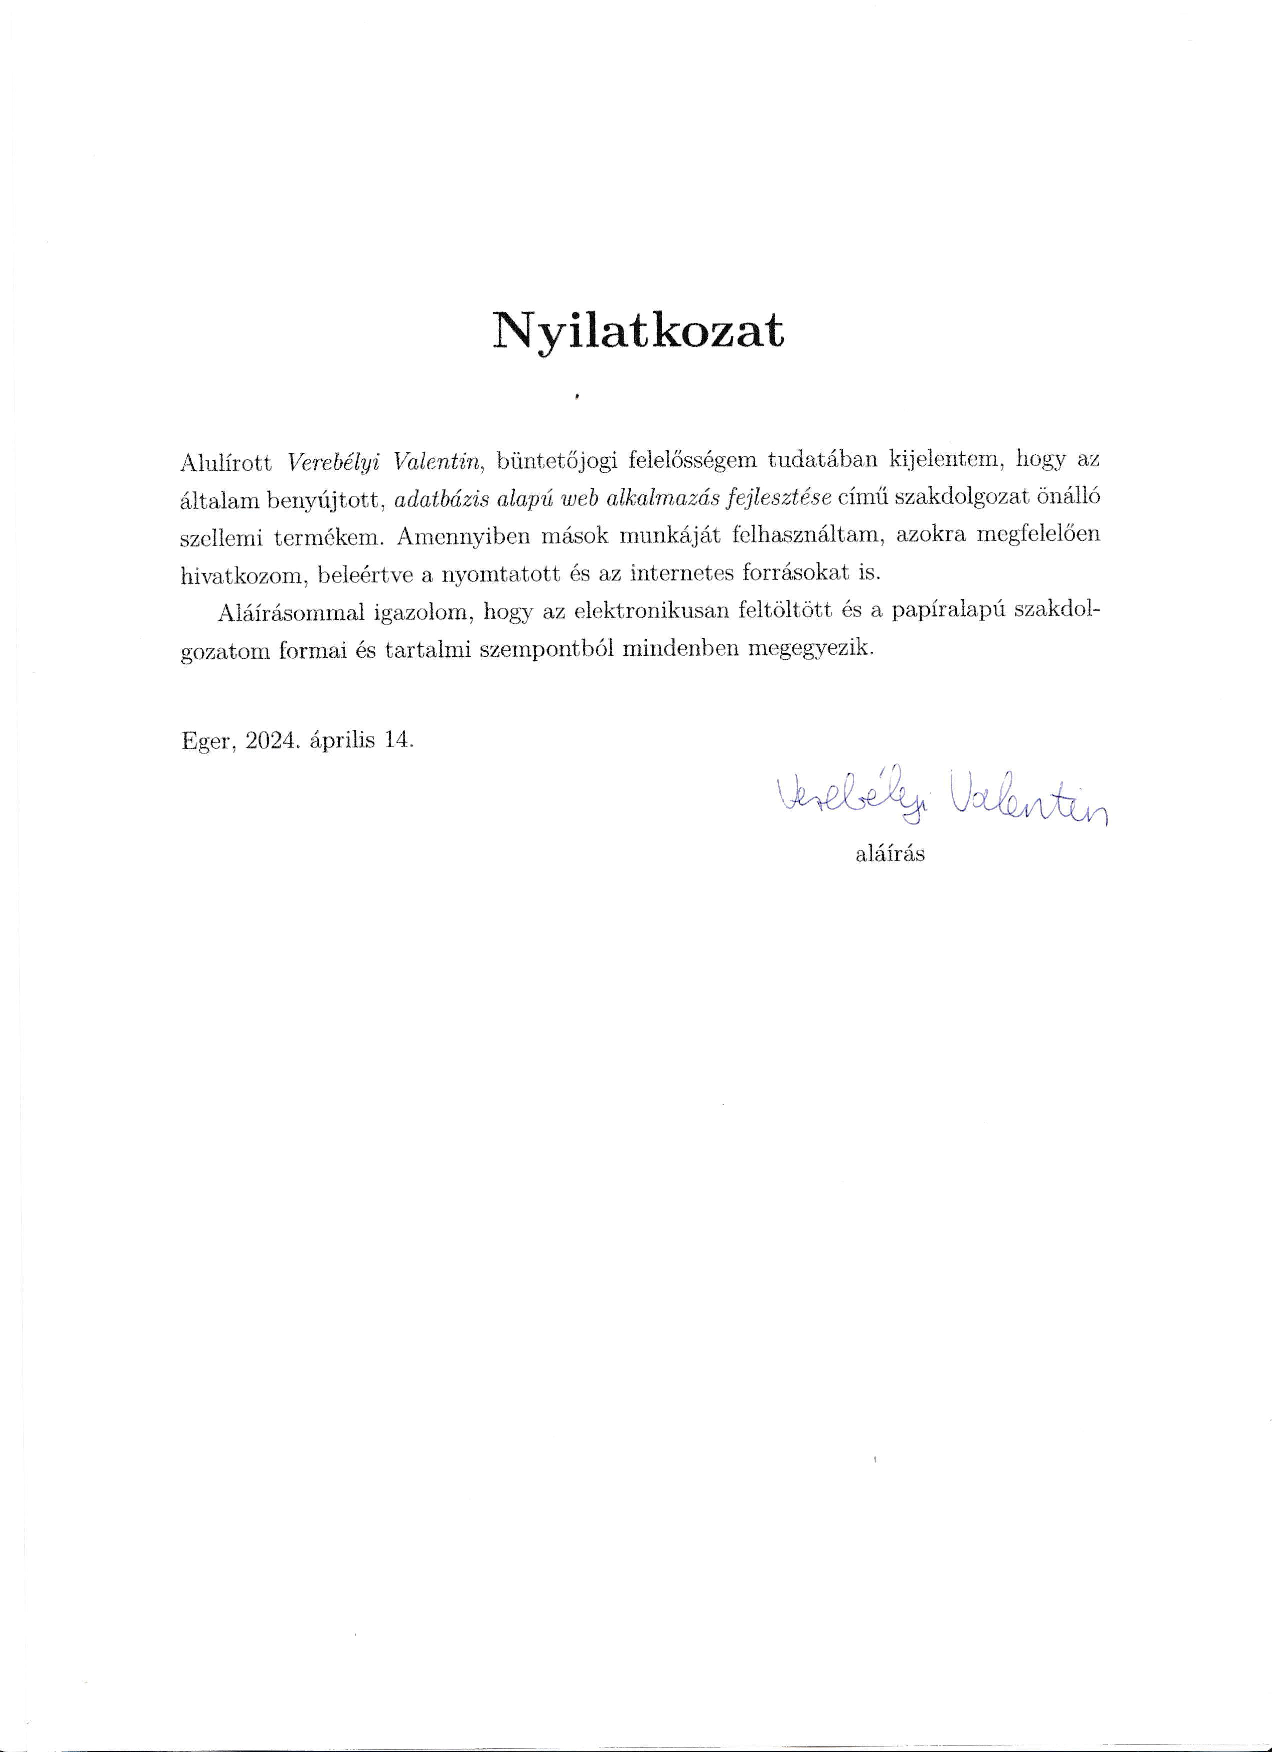
\includepdf{nyilatkozat.pdf}
\end{document}